Currently, we have adapted Persson and Peraire's method \cite{Persson06} for shock detection and capturing. The method works well for inviscid flow cases and compressible flows upto a Mach number of 2 have been tried and tested. However the method requires fine-tuning of parameters for each problem and we are currently working on a new method which is more robust. Persson and Peraire have used this shock capturing tool as a stabilization method as well in their turbulence calculations and we plan to test this and present results for inviscid and viscous cases in the final draft. Here we show a few inviscid results for the case of M = 1.6 where we illustrate the ability to detect shocks and add dissipation in a local manner in the form of artificial viscosity in order to capture the shock in a fine manner and avoid the loss of accuracy away from the shock.    

\begin{figure}[h] \tt
\centering
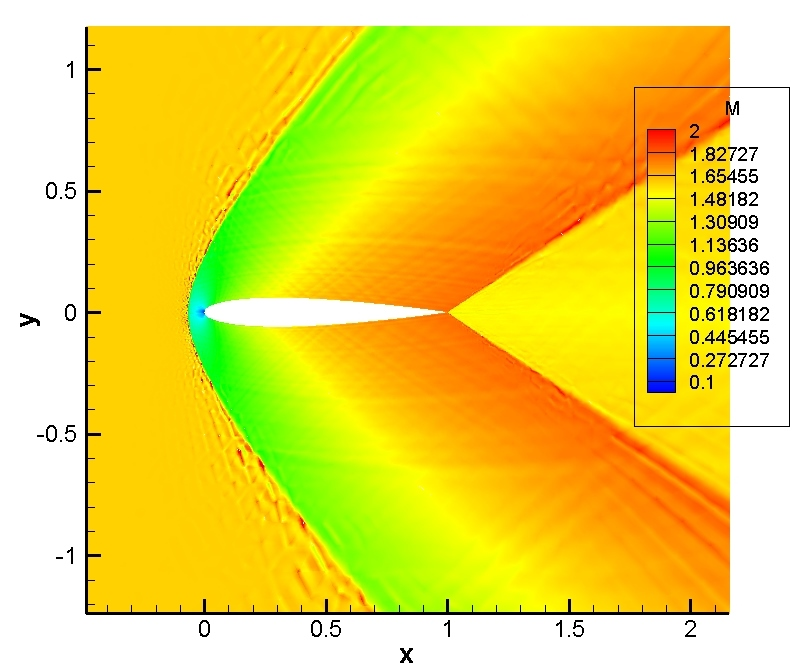
\includegraphics[angle=0, scale = 0.55]{./figures/M1pt6order3-inv-720ktime-mach.jpg} \\
\caption{Mach contours for inviscid flow over Naca0012 at M = 1.6 and AoA = $0^{\circ} $}
\label{fig:inv_mach}
\end{figure}

\begin{figure}
\centering
\begin{minipage}[t]{.5\textwidth}
  \centering
  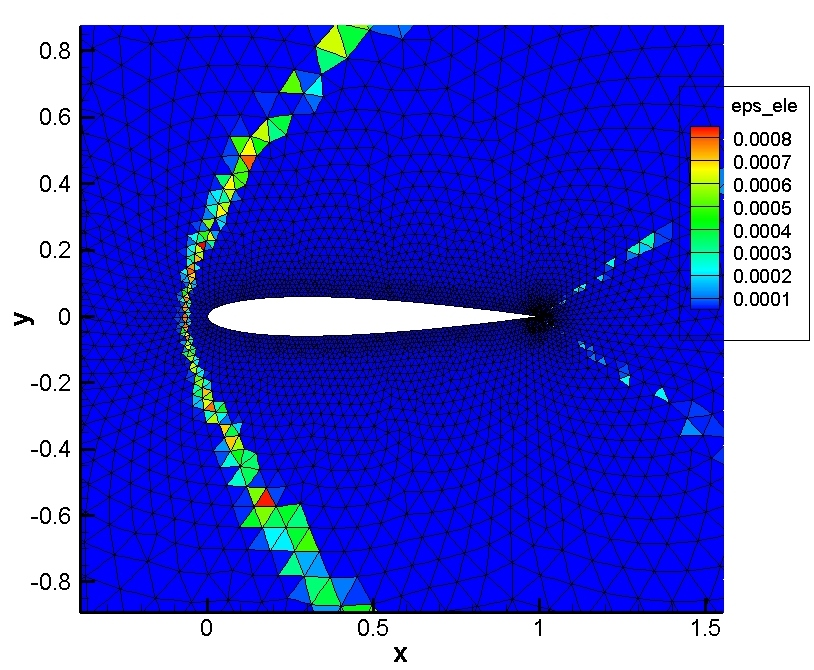
\includegraphics[width=.85\linewidth]{./figures/M1pt6-inv-av-ele-mesh}
  \captionof{figure}{Element-wise AV co-efficients (case 1)}
  \label{fig:AV-ele}
\end{minipage}%
\begin{minipage}[t]{.5\textwidth}
  \centering
  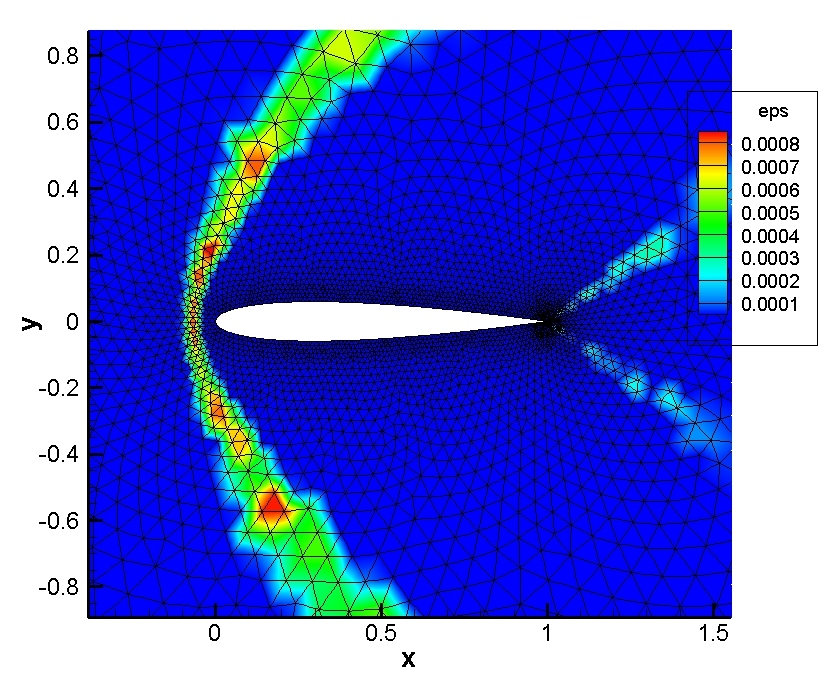
\includegraphics[width=.85\linewidth]{./figures/M1pt6-inv-av-mesh}
  \captionof{figure}{AV co-efficients with continuity enforcement}
  \label{fig:AV-cont}
\end{minipage}
\end{figure} 

